% Written by Daina Chiba (daina.chiba@gmail.com).
% It was mostly copied from two poster style files:
% beamerthemeI6pd2.sty written by
%	 	Philippe Dreuw <dreuw@cs.rwth-aachen.de> and
% 		Thomas Deselaers <deselaers@cs.rwth-aachen.de>
% and beamerthemeconfposter.sty written by
%     Nathaniel Johnston (nathaniel@nathanieljohnston.com)
%		http://www.nathanieljohnston.com/2009/08/latex-poster-template/
% ---------------------------------------------------------------------------------------------------%
% Preamble
% ---------------------------------------------------------------------------------------------------%
\documentclass[final]{beamer}
\usepackage[orientation=landscape,size=custom,width=110,height=86,scale=1.2,debug]{beamerposter}
\mode<presentation>{\usetheme{RicePoster}}
\usepackage[english]{babel}
\usepackage[latin1]{inputenc}
\usepackage[T1]{fontenc}
\usepackage{amsmath,amsthm, amssymb, latexsym}

\usepackage{array,booktabs,tabularx}
\newcolumntype{Z}{>{\centering\arraybackslash}X} % centered tabularx columns


%   Begin Additional Packages
\usepackage{blindtext}
%   End Additional Packages


% comment
\newcommand{\comment}[1]{}

\newlength{\columnheight}
\setlength{\columnheight}{80cm}
\newlength{\sepwid}
\newlength{\onecolwid}
\newlength{\twocolwid}
\newlength{\threecolwid}
\setlength{\sepwid}{0.024\paperwidth}
\setlength{\onecolwid}{0.24\paperwidth}
\setlength{\twocolwid}{0.4\paperwidth}
\setlength{\threecolwid}{0.19\paperwidth}

% ---------------------------------------------------------------------------------------------------%
% Title, author, date, etc.
% ---------------------------------------------------------------------------------------------------%
\title{\huge deton8: Detector of Nuclei}
\author{Will LeVine \& Gabriel Vacaliuc}
\institute[Rice University]{Department of Computer Science, Rice University}
\date[Apr.2018]{April, 2018}
\def\conference{COMP540 Term Project: 2018 Data Science Bowl}
\def\yourEmail{wvl1@rice.edu,gv8@rice.edu}


% ---------------------------------------------------------------------------------------------------%
% Contents
% ---------------------------------------------------------------------------------------------------%
\begin{document}
\begin{frame}[t]

\begin{columns}[t]

\begin{column}{\onecolwid}

    \begin{block}{Introduction}
        \blindtext
    \end{block}

    \vskip3ex

    \begin{block}{Preprocessing \& Data Whitening}
        \blindtext
    \end{block}

    \vskip3ex

    \begin{block}{Hand Designed Features}
      \begin{itemize}
        \item Bilateral Filter: convolves image with weighted Gaussian kernel; denoises
the image, while still preserving the edges
        \item 50/99 Image Rescaling: stretches pixel distribution; increases contrast between
        foreground and background
        \item Contrast Limited Adaptive Histogram Equalization: increases contrast locally;
        increases brightness of small nuclei
        \item Dilation: convolves image with uniform kernel; increases area of small nuclei
      \end{itemize}
    \end{block}

\end{column}

% -----------------------------------------------------------
% Start the second column
% -----------------------------------------------------------
\begin{column}{\twocolwid}
\begin{columns}[t,totalwidth=\twocolwid]
        \begin{column}{\threecolwid}
  % -----------------------------------------------------------
  % 2-1a
  % -----------------------------------------------------------
  \begin{block}{Sample Block (Left)}
    \baselineskip=.7\baselineskip

Put whatever you want.
\begin{itemize}
\item Yes.
\item This
\item is
\item just
\item an
\item example.
\end{itemize}

\vskip1ex
  \end{block}
    \end{column}
    \begin{column}{3.75ex}\end{column}
        \begin{column}{\threecolwid}

  % -----------------------------------------------------------
  % 2-1b
  % -----------------------------------------------------------
  \begin{block}{Sample Block (Right)}
    \baselineskip=.7\baselineskip

Put whatever you want.
\vspace{1ex}
\begin{itemize}
\item No.
\item This
\item is
\item not
\item a real
\item poster.
\end{itemize}
  \end{block}
    \end{column}
   \end{columns}
  \vskip2ex

  % -----------------------------------------------------------
  % 2-3
  % -----------------------------------------------------------
  \begin{alertblock}{Sample Block (Wide)}
\begin{columns}[c] \column{.45\textwidth}
%      \vskip1ex
  {\bf This block is wide.}
  \begin{itemize}
  \item Put something here.Put something here.Put something here.
  \item Put something here.Put something here.
  \item Don't you get it? Put something here.
  \end{itemize}

%\vskip2ex

% Phantom column
\column{.01\textwidth}
\begin{beamercolorbox}[wd=.1in,ht=2in]{cboxg}\end{beamercolorbox}
\vskip2ex

\column{.45\textwidth}
\vskip2ex
  {\bf Put something here.}
  \vskip1ex
\begin{tabular}{>{\color{myred}}rl}
Something & = Blur blur blur\\
    & Yadi Yadi Ya \\ [1em]
Anything & = Put something here. \\
    & OK?
\end{tabular}

\end{columns}

\vskip3ex

  {\bf Please}:
  Put something here.
    {\small
\begin{align}
{\cal L} &= \prod_{i=1}^{n}
\Pr(T_{wi} > t^0_{wi})^{(1-c_i)}
\Pr(T_{wi} = t_{wi} \cap T_{pi} > t^0_{pi} )^{c_i (1-d_i)}
\Pr(T_{wi} = t_{wi} \cap T_{pi} = t_{pi} )^{c_i d_i}. \nonumber
\end{align}
}

  \end{alertblock}

\vskip2ex

  % -----------------------------------------------------------
  % 2-3
  % -----------------------------------------------------------
  \begin{block}{Another Sample Block}
  \vskip-2ex
  \begin{figure}[h]
\hfill
\begin{minipage}[t]{.49\textwidth}
\begin{center}
\caption{Figure Title Here}
    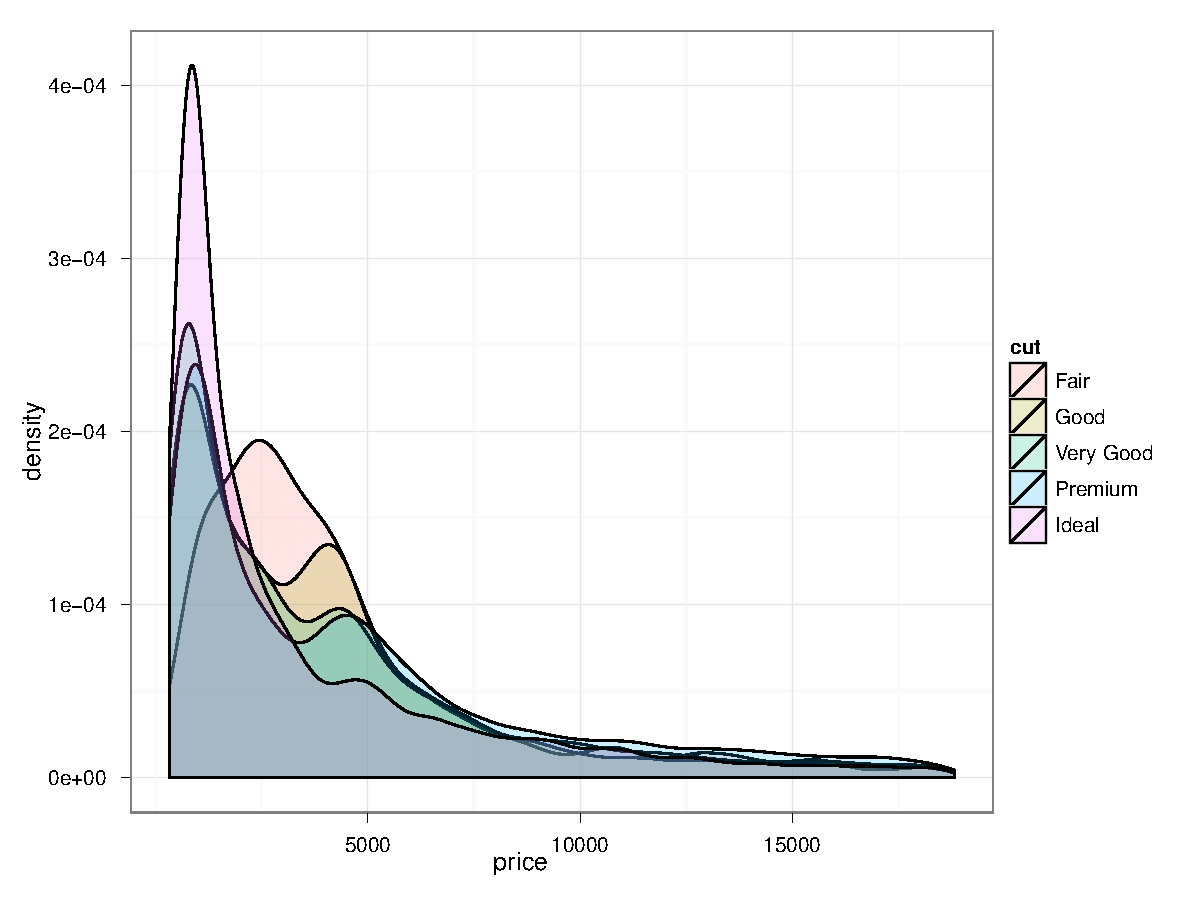
\includegraphics{./figs/figLeft}
\end{center}
\end{minipage}
\hfill
\begin{minipage}[t]{.49\textwidth}
\begin{center}
\caption{Figure Title Here}
    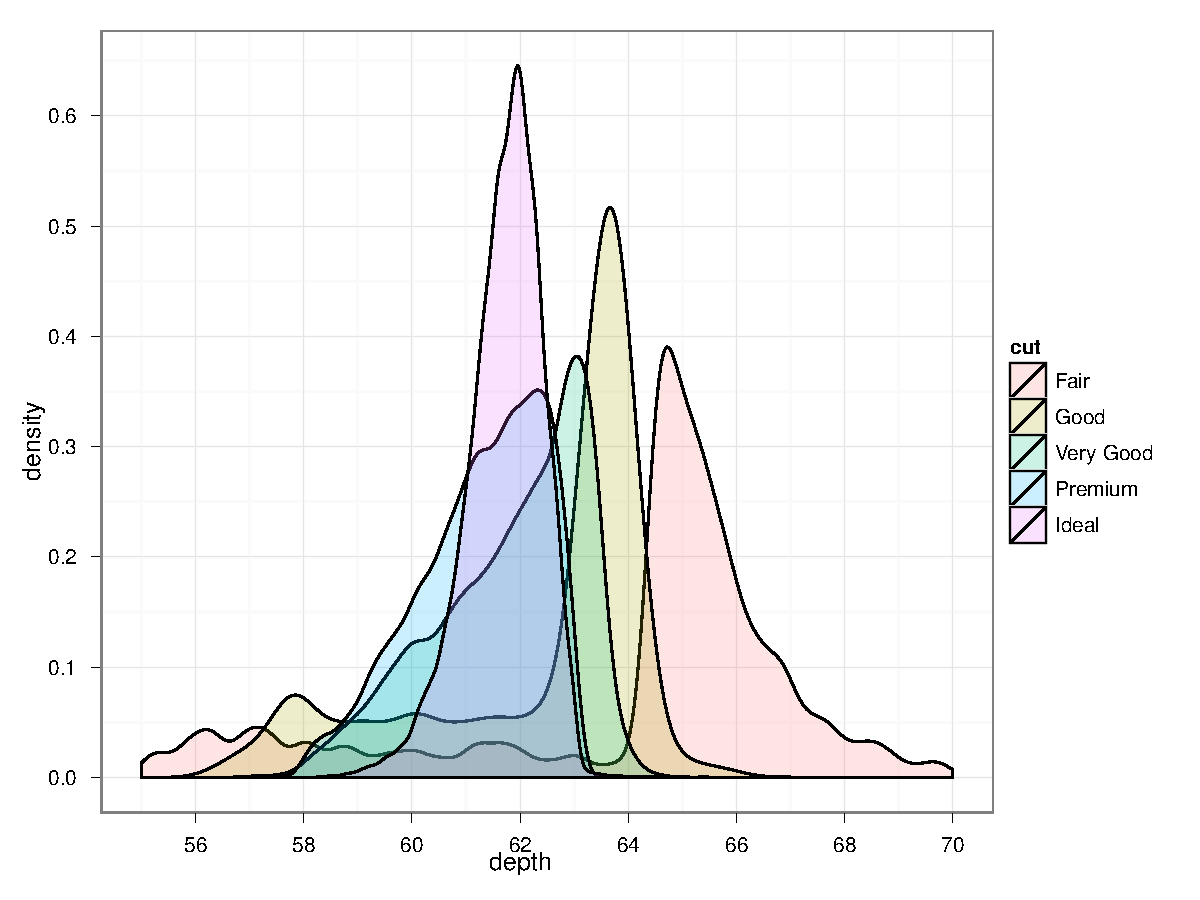
\includegraphics{./figs/figRight}
\end{center}
\end{minipage}
\hfill
\end{figure}
\vskip3ex

R code ({\tt plotFigs.R}) accompanying this template will produce all the figures included in this poster (except for the Rice Logo).

\vskip1ex

{\bf Explain the figure here.}
\begin{itemize}
\item Put something here. Put something here. Put something here. Put something here. Put something here.
\item Put something here. Put something here. Put something here. Put something here. Put something here.
\end{itemize}

\vskip3ex

{\bf Put something here.}
\begin{itemize}
\item Blur Blur Blur
\item Yadi Yadi Yah
\end{itemize}

  \end{block}

\end{column}

% -----------------------------------------------------------
% Start the third column
% -----------------------------------------------------------
\begin{column}{\onecolwid}
\vskip3ex

  % -----------------------------------------------------------
  % 3-0
  % -----------------------------------------------------------
  \begin{block}{Sample Block}
    \baselineskip=.7\baselineskip
\vskip2ex
    The following table is from the TeXShop template.

\vskip2ex

% Requires the booktabs if the memoir class is not being used
\begin{table}[htbp]
\centering
%\topcaption{Table captions are better up top} % requires the topcapt package
\begin{tabular}{@{} lcr @{}} % Column formatting, @{} suppresses leading/trailing space
  \toprule
  \multicolumn{2}{c}{Item} \\
  \cmidrule(r){1-2} % Partial rule. (r) trims the line a little bit on the right; (l) & (lr) also possible
  Animal    & Description & Price (\$)\\
  \midrule
  Gnat      & per gram & 13.65 \\
            & each     &  0.01 \\
  Gnu       & stuffed  & 92.50 \\
  Emu       & stuffed  & 33.33 \\
  Armadillo & frozen   &  8.99 \\
  \bottomrule
\end{tabular}
\caption{Remember, \emph{never} use vertical lines in tables.}
\label{tab:booktabs}
\end{table}

\vskip2ex

{\bf I honestly don't know what this table means.}
\begin{itemize}
\item This is just
\item an
\item example.
\end{itemize}

  \end{block}

\vskip3ex


  % -----------------------------------------------------------
  % 3-4
  % -----------------------------------------------------------
  \begin{alertblock}{Findings}
    \baselineskip=.7\baselineskip

  \vskip2ex

\begin{figure}
\begin{center}
\caption{Effect of X on Y}
    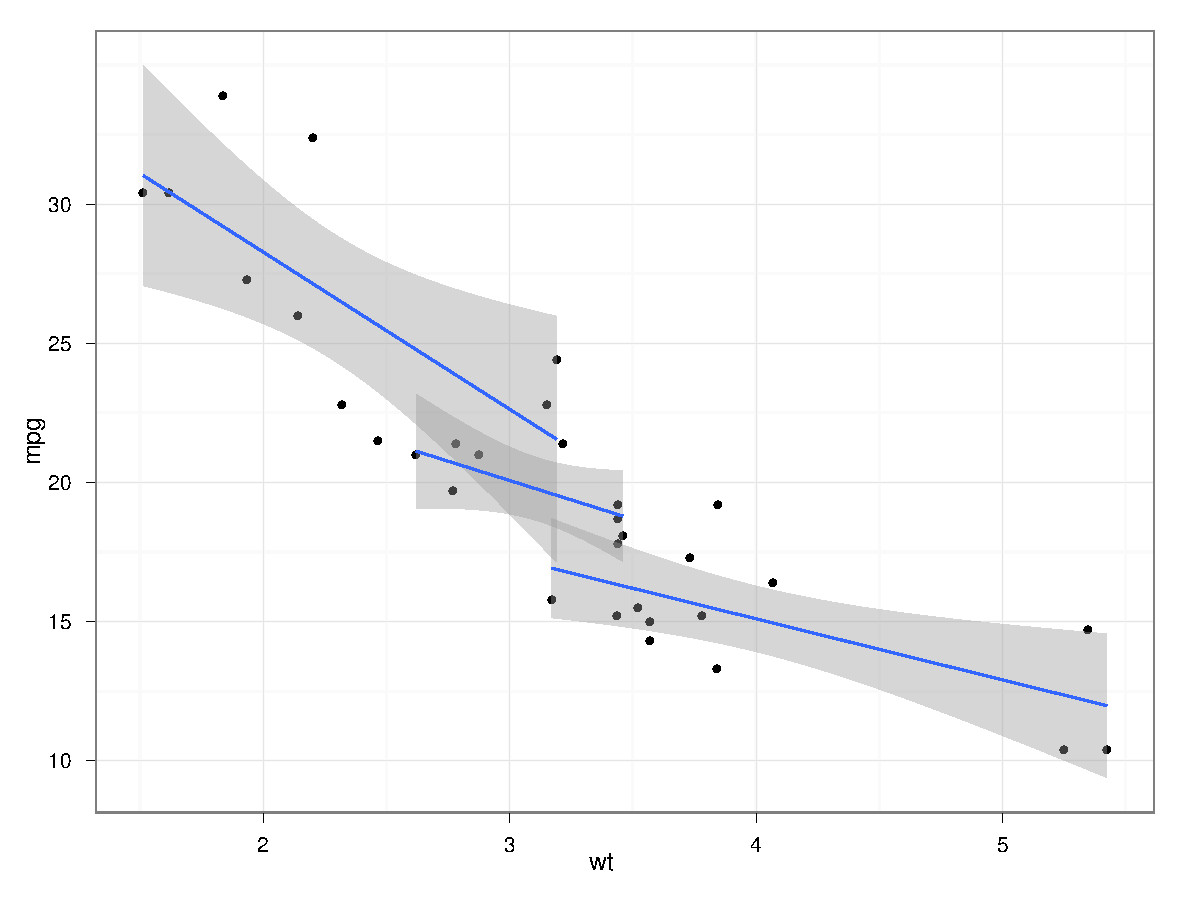
\includegraphics{./figs/figResult}
\end{center}
\end{figure}
Explain the findings.
  \vskip2ex

\end{alertblock}
  \vskip2ex

  % -----------------------------------------------------------
  % 3-4
  % -----------------------------------------------------------
  \begin{block}{Conclusion}
    \baselineskip=.7\baselineskip

  \vskip2ex

{\bf Remember:}\\
\begin{itemize}
\item You'd
\item better
\item keep
\item it
\item simple!
\end{itemize}

  \vskip2ex

\end{block}
  \vskip2ex


\end{column}
\end{columns}
\end{frame}
\end{document}
